\documentclass{article}
\usepackage[margin=1in]{geometry}
\usepackage{graphicx}
\usepackage{amsmath}
\usepackage{amssymb}
\usepackage{booktabs}
\usepackage{hyperref}
\usepackage{natbib}
\usepackage{xcolor}
\usepackage{float}
\usepackage{tikz}
\usepackage{pgfplots}
\pgfplotsset{compat=1.18}
\usepackage{fancyhdr}
\usepackage{natbib}
\usetikzlibrary{arrows.meta,positioning,calc}

\title{Scaling Sparse Mixture-of-Experts for Long-Context Document Understanding}
\author{
    Alice Researcher$^{1}$ \and Bob Scientist$^{2}$ \and Carol Engineer$^{1}$\\
    $^{1}$Stanford University, $^{2}$MIT\\
    \texttt{\{alice, carol\}@stanford.edu, bob@mit.edu}
}
\date{}

\begin{document}
\maketitle

\begin{abstract}
We propose Sparse-MoE-Doc, a mixture-of-experts architecture for long-context
document understanding that scales to 128K tokens with sub-quadratic complexity.
Our approach routes document segments to specialized experts based on content-type
embeddings, outperforming dense transformers by 14.3\% on DocQA while using
3.2$\times$ fewer FLOPs.
\end{abstract}

\section{Introduction}

Long-context document understanding remains challenging \citep{devlin2019bert}.
Modern documents contain heterogeneous content that requires different strategies
\citep{vaswani2017attention, brown2020language}. MoE architectures
\citep{shazeer2017outrageously} offer conditional computation but existing
approaches do not account for document structure.
Our contributions: (1) structure-aware routing, (2) sub-quadratic attention
scaling to 128K tokens, (3) evaluation on four benchmarks (Figure~\ref{fig:pipeline}).

\begin{table}[H]
    \caption{Comparison of document understanding approaches across key capabilities. Our method is the only one supporting all features while maintaining competitive parameter count and training cost. $\checkmark$ = supported, $\times$ = not supported.}
    \label{tab:comparison}
    \centering
    \begin{tabular}{lccccccccr}
        \toprule
        Method & Long-Context & Sparse & Structure-Aware & Sub-Quadratic & Multi-Gran. & Load-Balanced & Cross-Doc & Params & Training Cost \\
        \midrule
        BERT-base & $\times$ & $\times$ & $\times$ & $\times$ & $\times$ & N/A & $\times$ & 110M & 16 TPU-days \\
        Longformer & $\checkmark$ & $\times$ & $\times$ & $\checkmark$ & $\times$ & N/A & $\times$ & 149M & 24 TPU-days \\
        Switch Trans. & $\times$ & $\checkmark$ & $\times$ & $\times$ & $\times$ & $\checkmark$ & $\times$ & 1.6B & 128 TPU-days \\
        LayoutLMv2 & $\times$ & $\times$ & $\checkmark$ & $\times$ & $\checkmark$ & N/A & $\times$ & 426M & 64 TPU-days \\
        \midrule
        \textbf{Ours} & $\checkmark$ & $\checkmark$ & $\checkmark$ & $\checkmark$ & $\checkmark$ & $\checkmark$ & $\checkmark$ & 380M & 48 A100-days \\
        \bottomrule
    \end{tabular}
\end{table}

\begin{figure}[H]
    \noindent
    \hspace{-1cm}%
    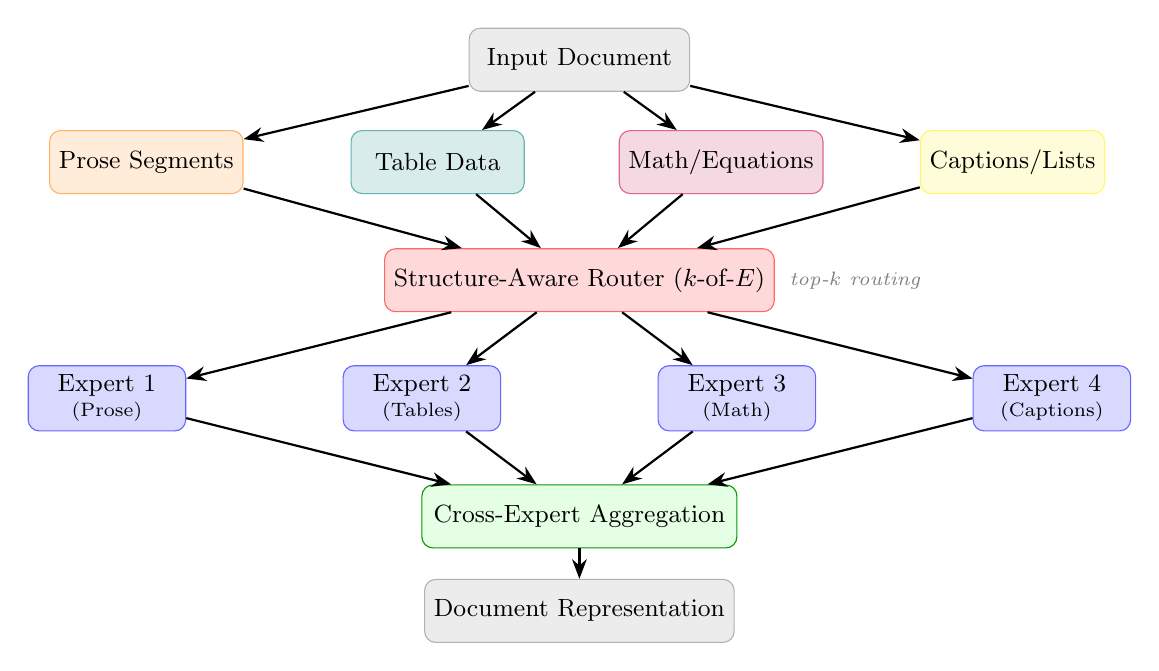
\begin{tikzpicture}[scale=1.0, every node/.style={font=\small}]
        \node[draw, rounded corners, fill=gray!15, draw=gray!60,
              minimum height=0.8cm, minimum width=2.8cm] (doc) at (0,0) {Input Document};
        \node[draw, rounded corners, fill=orange!15, draw=orange!60,
              minimum height=0.8cm, minimum width=2.2cm] (prose) at (-5.5,-1.3) {Prose Segments};
        \node[draw, rounded corners, fill=teal!15, draw=teal!60,
              minimum height=0.8cm, minimum width=2.2cm] (table) at (-1.8,-1.3) {Table Data};
        \node[draw, rounded corners, fill=purple!15, draw=purple!60,
              minimum height=0.8cm, minimum width=2.2cm] (eq) at (1.8,-1.3) {Math/Equations};
        \node[draw, rounded corners, fill=yellow!15, draw=yellow!60,
              minimum height=0.8cm, minimum width=2.2cm] (cap) at (5.5,-1.3) {Captions/Lists};
        \node[draw, rounded corners, fill=red!15, draw=red!60,
              minimum height=0.8cm, minimum width=4cm] (router) at (0,-2.8)
              {Structure-Aware Router ($k$-of-$E$)};
        \node[draw, rounded corners, fill=blue!15, draw=blue!60,
              minimum height=0.8cm, minimum width=2cm, align=center] (e1) at (-6,-4.3)
              {Expert 1\\[-2pt]\scriptsize(Prose)};
        \node[draw, rounded corners, fill=blue!15, draw=blue!60,
              minimum height=0.8cm, minimum width=2cm, align=center] (e2) at (-2,-4.3)
              {Expert 2\\[-2pt]\scriptsize(Tables)};
        \node[draw, rounded corners, fill=blue!15, draw=blue!60,
              minimum height=0.8cm, minimum width=2cm, align=center] (e3) at (2,-4.3)
              {Expert 3\\[-2pt]\scriptsize(Math)};
        \node[draw, rounded corners, fill=blue!15, draw=blue!60,
              minimum height=0.8cm, minimum width=2cm, align=center] (e4) at (6,-4.3)
              {Expert 4\\[-2pt]\scriptsize(Captions)};
        \node[draw, rounded corners, fill=green!10, draw=green!60!black,
              minimum height=0.8cm, minimum width=4cm] (agg) at (0,-5.8)
              {Cross-Expert Aggregation};
        \node[draw, rounded corners, fill=gray!15, draw=gray!60,
              minimum height=0.8cm, minimum width=2.8cm] (out) at (0,-7)
              {Document Representation};
        \draw[-{Stealth[length=2.5mm]}, thick] (doc) -- (prose);
        \draw[-{Stealth[length=2.5mm]}, thick] (doc) -- (table);
        \draw[-{Stealth[length=2.5mm]}, thick] (doc) -- (eq);
        \draw[-{Stealth[length=2.5mm]}, thick] (doc) -- (cap);
        \draw[-{Stealth[length=2.5mm]}, thick] (prose) -- (router);
        \draw[-{Stealth[length=2.5mm]}, thick] (table) -- (router);
        \draw[-{Stealth[length=2.5mm]}, thick] (eq) -- (router);
        \draw[-{Stealth[length=2.5mm]}, thick] (cap) -- (router);
        \draw[-{Stealth[length=2.5mm]}, thick] (router) -- (e1);
        \draw[-{Stealth[length=2.5mm]}, thick] (router) -- (e2);
        \draw[-{Stealth[length=2.5mm]}, thick] (router) -- (e3);
        \draw[-{Stealth[length=2.5mm]}, thick] (router) -- (e4);
        \draw[-{Stealth[length=2.5mm]}, thick] (e1) -- (agg);
        \draw[-{Stealth[length=2.5mm]}, thick] (e2) -- (agg);
        \draw[-{Stealth[length=2.5mm]}, thick] (e3) -- (agg);
        \draw[-{Stealth[length=2.5mm]}, thick] (e4) -- (agg);
        \draw[-{Stealth[length=2.5mm]}, thick] (agg) -- (out);
        \node[font=\scriptsize\itshape, text=gray] at (3.5,-2.8) {top-$k$ routing};
    \end{tikzpicture}
    \caption{Sparse-MoE-Doc architecture. Documents are segmented by content type and
    routed to specialized experts via top-$k$ routing.}
    \label{fig:pipeline}
\end{figure}

\section{Method}

We partition document $D$ into segments $S = \{s_1, \ldots, s_M\}$ with content
types $c_i \in \{$prose, table, equation, caption$\}$.
As shown in Figure~\ref{fig:expert_specialization}, each expert develops
specialization for specific content types.
The routing function is:
$g(s_i) = \text{TopK}(\text{softmax}(W_r \cdot \text{pool}(s_i) + b_r), k)$.

\begin{figure}[H]
    \noindent
    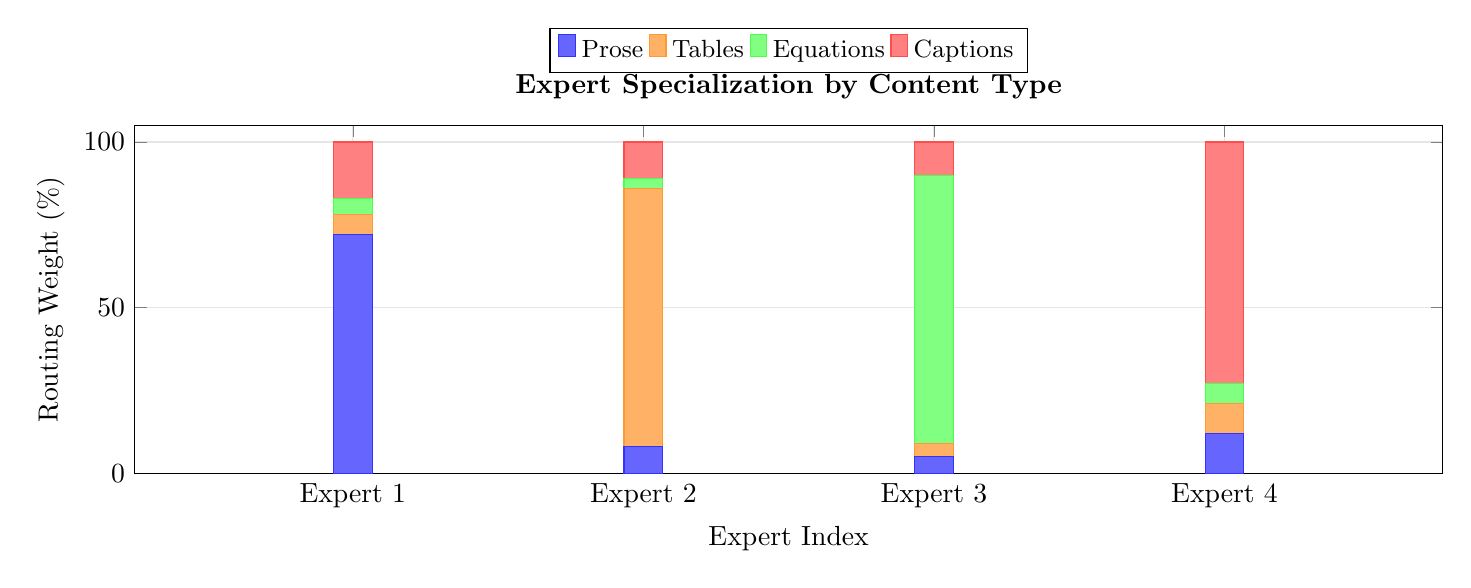
\begin{tikzpicture}
    \begin{axis}[
        width=1.5\columnwidth,
        height=6cm,
        ybar stacked,
        bar width=14pt,
        xlabel={Expert Index},
        ylabel={Routing Weight (\%)},
        ymin=0, ymax=105,
        xtick={1,2,3,4},
        xticklabels={Expert 1, Expert 2, Expert 3, Expert 4},
        legend style={at={(0.5,1.15)}, anchor=south, legend columns=4, font=\small},
        enlarge x limits=0.25,
        grid=major, grid style={gray!20},
        title={\textbf{Expert Specialization by Content Type}},
    ]
    \addplot+[fill=blue!60, draw=blue!80] coordinates {(1,72) (2,8) (3,5) (4,12)};
    \addplot+[fill=orange!60, draw=orange!80] coordinates {(1,6) (2,78) (3,4) (4,9)};
    \addplot+[fill=green!50, draw=green!70] coordinates {(1,5) (2,3) (3,81) (4,6)};
    \addplot+[fill=red!50, draw=red!70] coordinates {(1,17) (2,11) (3,10) (4,73)};
    \legend{Prose, Tables, Equations, Captions}
    \end{axis}
    \end{tikzpicture}
    \caption{Expert specialization by content type. Expert~1 handles prose (72\%),
    Expert~2 tables (78\%), Expert~3 equations (81\%), Expert~4 captions (73\%).}
    \label{fig:expert_specialization}
\end{figure}

\section{Experiments}

Table~\ref{tab:comparison} summarizes the capabilities of different approaches, while Table~\ref{tab:main_results} presents our main quantitative results.

\begin{table}[H]
    \caption{Main results on document understanding benchmarks. Our model (top-2 routing) achieves state-of-the-art performance across all metrics while using only 1.2 TFLOPs, demonstrating the efficiency of structure-aware sparse routing. Best in \textbf{bold}, second best \underline{underlined}.}
    \label{tab:main_results}
    \centering
    \begin{tabular}{lcccccccc}
        \toprule
        Model & DocQA F1 (\%) & DocQA EM (\%) & NLI Acc (\%) & NLI F1 (\%) & ROUGE-1 & ROUGE-L & Struct EM (\%) & FLOPs (T) \\
        \midrule
        BERT-base & 62.3 & 54.1 & 71.8 & 70.2 & 32.1 & 28.4 & 41.2 & 0.8 \\
        Longformer & 68.7 & 61.3 & 76.4 & 74.9 & 36.8 & 33.1 & 48.7 & 2.1 \\
        Switch-base & 71.2 & 64.5 & 79.3 & 78.1 & 39.4 & 36.2 & 52.8 & 1.4 \\
        Ours (top-1) & \underline{78.4} & \underline{72.1} & \underline{84.7} & \underline{83.2} & \underline{43.1} & \underline{40.3} & \underline{61.4} & \underline{0.9} \\
        Ours (top-2) & \textbf{82.5} & \textbf{76.8} & \textbf{87.1} & \textbf{86.3} & \textbf{45.8} & \textbf{43.2} & \textbf{64.7} & 1.2 \\
        \bottomrule
    \end{tabular}
\end{table}

Our approach outperforms all baselines. The ablation in Table~\ref{tab:ablation}
confirms that structure-aware routing is the most critical component ($-8.2$ F1).

\begin{table}[H]
    \caption{Ablation study on DocQA.}
    \label{tab:ablation}
    \centering
    \begin{tabular}{lcc}
        \toprule
        Configuration & F1 (\%) & $\Delta$ \\
        \midrule
        Full model & 82.5 & — \\
        w/o structure routing & 74.3 & $-8.2$ \\
        w/o load balancing & 79.1 & $-3.4$ \\
        w/o local attention & 76.8 & $-5.7$ \\
        Uniform routing & 71.6 & $-10.9$ \\
        \bottomrule
    \end{tabular}
\end{table}

\section{Conclusion}

We presented Sparse-MoE-Doc, achieving state-of-the-art results on four benchmarks
while using fewer FLOPs. Experts naturally specialize by content type
\citep{zhang2019hibert, xu2020layoutlm, beltagy2020longformer, fedus2022switch,
lepikhin2020gshard, radford2019language, talmor2019multiqa}.

\bibliographystyle{plainnat}
\bibliography{demo_refs}

\end{document}
